% Beamer deck. Numbers come from ../report/numbers.tex (generated from results/*.json). Draft prepared with an AI assistant;
% the student must revise it in their own words and be able to explain every slide (handout rule on slides).
\documentclass[aspectratio=169,10pt,t]{beamer}
\usetheme{Madrid}
\definecolor{navy}{HTML}{1F3A5F}
\definecolor{accent}{HTML}{2A78D6}
\definecolor{warn}{HTML}{EB6834}
\definecolor{ink}{HTML}{0B0B0B}
\setbeamercolor{structure}{fg=navy}
\setbeamercolor{palette primary}{bg=navy,fg=white}
\setbeamercolor{palette secondary}{bg=navy!85!white,fg=white}
\setbeamercolor{palette tertiary}{bg=navy!70!white,fg=white}
\setbeamercolor{block title}{bg=navy,fg=white}
\setbeamercolor{block body}{bg=navy!6!white}
\setbeamercolor{alerted text}{fg=warn}
\setbeamertemplate{navigation symbols}{}
\setbeamertemplate{footline}{\hfill\insertframenumber/\inserttotalframenumber\hspace{0.4cm}\vspace{0.2cm}}
\setbeamerfont{block title}{size=\small}
\setbeamerfont{frametitle}{size=\large}
\usepackage{amsmath,amssymb,booktabs,graphicx,tikz,xcolor,microtype}
\usetikzlibrary{arrows.meta,positioning,shapes.geometric}
\graphicspath{{../report/}}
% GENERATED by scripts/build_report_assets.py from results/*.json - do not edit
\newcommand{\officialRows}{0 & 0.972 & 46.57 & 7.3 & 0.796 & 0.419 & 0.00\% & 15 \\
101 & 0.975 & 46.84 & 7.3 & 0.808 & 0.416 & 0.00\% & 15 \\
202 & 0.970 & 46.47 & 7.1 & 0.801 & 0.433 & 0.00\% & 15 \\
303 & 0.973 & 47.05 & 6.8 & 0.748 & 0.445 & 0.00\% & 15 \\
404 & 0.964 & 46.79 & 7.0 & 0.780 & 0.425 & 0.00\% & 15 \\}
\newcommand{\chkDet}{yes}
\newcommand{\chkSeed}{yes}
\newcommand{\chkMixed}{0.96}
\newcommand{\chkSingle}{0.95}
\newcommand{\manifestRows}{8{,}029}
\newcommand{\params}{5{,}098{,}915}
\newcommand{\sizeMB}{19.8}
\newcommand{\sampleSpeed}{18}
\newcommand{\trainHours}{1.3}
\newcommand{\nSeeds}{61}
\newcommand{\nFifteen}{60}
\newcommand{\nBelow}{1}
\newcommand{\recallMean}{0.433}
\newcommand{\recallMin}{0.395}
\newcommand{\recallMax}{0.488}
\newcommand{\fidMean}{46.72}
\newcommand{\fidMin}{46.14}
\newcommand{\fidMax}{47.35}
\newcommand{\accMean}{0.971}
\newcommand{\accMin}{0.962}
\newcommand{\accMax}{0.979}
\newcommand{\precMean}{0.785}
\newcommand{\precMin}{0.746}
\newcommand{\precMax}{0.814}
\newcommand{\recallSD}{0.019}
\newcommand{\memMax}{0.00}
\newcommand{\lowSeed}{31415}
\newcommand{\lowRecall}{0.3949}
\newcommand{\lowZ}{2.0}
\newcommand{\pFifteen}{98.4}
\newcommand{\pFifteenLo}{91.3}
\newcommand{\pFifteenHi}{99.7}
\newcommand{\wideAtFifteen}{12}
\newcommand{\wideRecall}{0.416}
\newcommand{\widePrec}{0.829}
\newcommand{\wideAcc}{0.979}
\newcommand{\smallAtFifteen}{15}
\newcommand{\smallRecall}{0.433}
\newcommand{\smallPrec}{0.788}
\newcommand{\smallAcc}{0.972}
\newcommand{\progressRows}{v009 & 1{,}399 & 12 / -- / -- & 0.936 & 60.6 & 0.333 & 0.759 & 4.35\% \\
v010 & 1{,}929 & 13 / -- / -- & 0.942 & 58.0 & 0.319 & 0.769 & 1.65\% \\
v010 + mirror & 1{,}929 & 14 / 13 / 13 & 0.954 & 50.6 & 0.388 & 0.768 & 0.00\% \\
v011 & 5{,}536 & 15 / 14 / 15 & 0.981 & 48.5 & 0.401 & 0.819 & 0.00\% \\
v012 & 4{,}610 & 14 / 14 / 15 & 0.976 & 48.0 & 0.381 & 0.828 & 0.00\% \\
v013 & 4{,}922 & 14 / -- / -- & 0.975 & 49.0 & 0.353 & 0.837 & 0.00\% \\
v014 (final) & 8{,}029 & 15 / 15 / 15 & 0.972 & 46.6 & 0.423 & 0.802 & 0.00\% \\}
\newcommand{\auditGood}{160}
\newcommand{\auditPct}{80.0}
\newcommand{\auditCI}{73.9--85.0}
\newcommand{\auditCat}{63/75}
\newcommand{\auditCatPct}{84.0}
\newcommand{\auditDog}{97/125}
\newcommand{\auditDogPct}{77.6}
\newcommand{\auditPersonal}{43/49}
\newcommand{\auditAI}{117/151}
\newcommand{\auditEars}{33}
\newcommand{\auditBad}{40}
\newcommand{\auditRecrop}{7/18}

\setlength{\parskip}{2pt}
\renewcommand{\arraystretch}{1.08}
\title[Cat and dog head generation]{Cat and Dog Head Generation from a Self-Curated Pool}
\subtitle{Data curation, a pixel-space diffusion model, and working with coding agents}
\author[Sou Chak Tong]{Sou Chak Tong\\[2pt]\small Student ID U-C3-2652-3}
\institute[CISC3024]{CISC3024 Pattern Recognition Project}
\date{26 November 2026}

\newcommand{\tile}[3]{% width, label, value  (stat tile)
  \begin{tikzpicture}\node[draw=navy,fill=navy!6!white,rounded corners=3pt,minimum width=#1,minimum height=1.25cm,align=center,inner sep=3pt]
  {{\Large\bfseries\color{navy}#3}\\[-1pt]{\scriptsize #2}};\end{tikzpicture}}

\begin{document}
\begin{frame}[plain]\titlepage\end{frame}

% ------------------------------------------------------------------------------------------------------------------ 2
\begin{frame}{Result at a glance}
\centering
\tile{2.62cm}{marks, official seed 0}{15 / 15}\hspace{3pt}
\tile{2.62cm}{seeds at 15 marks}{\nFifteen{} of \nSeeds}\hspace{3pt}
\tile{2.62cm}{FID (seed 0), limit 50}{46.6}\hspace{3pt}
\tile{2.62cm}{recall (seed 0), limit 0.40}{0.419}\hspace{3pt}
\tile{2.62cm}{personal audit: crops good}{\auditPct\,\%}

\vspace{0.2cm}
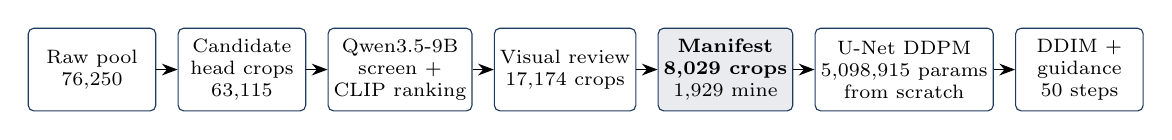
\begin{tikzpicture}[node distance=0.27cm,every node/.style={draw=navy,fill=white,rounded corners=2pt,align=center,font=\scriptsize,minimum height=1.05cm,minimum width=1.62cm,inner sep=2pt},
  >={Stealth[length=2mm]}]
\node (a) {Raw pool\\76{,}250};
\node (b) [right=of a] {Candidate\\head crops\\63{,}115};
\node (c) [right=of b] {Qwen3.5-9B\\screen +\\CLIP ranking};
\node (d) [right=of c] {Visual review\\17{,}174 crops};
\node (e) [right=of d,fill=navy!10!white] {\textbf{Manifest}\\\textbf{8{,}029 crops}\\1{,}929 mine};
\node (f) [right=of e] {U-Net DDPM\\\params{} params\\from scratch};
\node (g) [right=of f] {DDIM +\\guidance\\50 steps};
\draw[->] (a)--(b); \draw[->] (b)--(c); \draw[->] (c)--(d); \draw[->] (d)--(e); \draw[->] (e)--(f); \draw[->] (f)--(g);
\end{tikzpicture}

\vspace{0.15cm}
\begin{columns}[T]
\begin{column}{0.48\linewidth}
\begin{block}{What worked}
\footnotesize\begin{itemize}\setlength{\itemsep}{0pt}
\item Mirroring exact crops: memorization 1.65\,\% $\to$ 0\,\%
\item More \emph{valid} images: recall 0.32 $\to$ 0.42
\item EMA, 16$\times$16 attention, PAG and FreeU guidance
\end{itemize}
\end{block}
\end{column}
\begin{column}{0.48\linewidth}
\begin{block}{What I want you to remember}
\footnotesize\begin{itemize}\setlength{\itemsep}{0pt}
\item Recall is the thin margin: seed \lowSeed{} gives 14/15
\item My audit: ears cut in 33 of 40 bad crops, missed by the agent
\item Metrics hide distortion: 39 of 128 samples unrecognizable
\end{itemize}
\end{block}
\end{column}
\end{columns}
\end{frame}

% ------------------------------------------------------------------------------------------------------------------ 3
\begin{frame}{Data pipeline: from 76{,}250 web images to 8{,}029 training crops}
\begin{columns}[T]
\begin{column}{0.56\linewidth}
\footnotesize
\begin{tabular}{@{}p{5.9cm}r@{}}
\toprule
Step & Images \\
\midrule
Raw pool (LAION, with other animals and scenes) & 76{,}250 \\
Candidate crops (detector squares, geometry rescue, rescue of misses) & 63{,}115 \\
Passed the Qwen3.5-9B screen & 6{,}718 \\
Agent visual review: reviewed / valid & 17{,}174 / 7{,}083 \\
Minus same-photo, duplicate, holdout rows & 6{,}100 \\
Plus my personally reviewed crops (50 batches) & 1{,}929 \\
\midrule
\textbf{Final manifest} (3{,}096 cat, 4{,}933 dog) & \textbf{\manifestRows} \\
Pool-only holdout (31 cat, 32 dog) & 63 \\
\bottomrule
\end{tabular}

\vspace{4pt}\footnotesize The review also covered crops the screen rejected, so the rows are not a strict funnel.
\end{column}
\begin{column}{0.42\linewidth}
\begin{block}{Handout rules every crop must meet}
\footnotesize\begin{itemize}\setlength{\itemsep}{0pt}
\item real photo, no cartoon, toy or print
\item exactly one head, centred, roughly upright
\item head with ears 60--80\,\% of the square
\item head $\ge$ 32 px wide in the pool image
\end{itemize}
\end{block}
\begin{block}{Boundaries I kept}
\footnotesize\begin{itemize}\setlength{\itemsep}{0pt}
\item official crop geometry, no padding, exact crops only
\item pretrained models used for curation only
\item no dev images, no evaluator networks
\item agent verdicts $\neq$ my verdicts; the audit is mine
\end{itemize}
\end{block}
\end{column}
\end{columns}
\end{frame}

% ------------------------------------------------------------------------------------------------------------------ 4
\begin{frame}{My audit: 200 crops, labelled without seeing the agent's verdicts}
\centering\includegraphics[width=0.93\linewidth]{fig_audit.pdf}

\vspace{2pt}
\begin{columns}[T]
\begin{column}{0.48\linewidth}
\begin{alertblock}{Finding}
\small \textbf{\auditGood{} of 200 good (\auditPct\,\%)}, 95\,\% interval \auditCI\,\%. \auditEars{} of \auditBad{} bad crops have \textbf{ears cut}, worst in re-cropped squares (\auditRecrop).
\end{alertblock}
\end{column}
\begin{column}{0.48\linewidth}
\begin{block}{Cause and next step}
\small Face-only detector boxes and ear margins judged on thumbnails. Next: re-review at 300 px with an explicit ear check, retrain, redraw the audit.
\end{block}
\end{column}
\end{columns}
\end{frame}

% ------------------------------------------------------------------------------------------------------------------ 5
\begin{frame}{Model and sampler}
\begin{columns}[T]
\begin{column}{0.49\linewidth}
\begin{block}{Conditional pixel U-Net, trained from scratch}
\small\begin{itemize}\setlength{\itemsep}{1pt}
\item $3{\times}32{\times}32$ in $[-1,1]$; widths 32/64/96/128; \params{} parameters
\item GroupNorm, SiLU, self-attention at 8$\times$8, 4$\times$4 and an added 16$\times$16 layer
\item condition = time MLP + class embedding (cat, dog, \emph{null}); scale and shift in each block
\item AdamW $2{\times}10^{-4}$, batch 128, bf16, EMA 0.9995, mirror $p{=}0.5$, label dropout 0.1
\end{itemize}
\[
x_t=\sqrt{\bar\alpha_t}\,x_0+\sqrt{1-\bar\alpha_t}\,\epsilon,\qquad
\mathcal L=\mathbb E\big\|\epsilon_\theta(x_t,t,\tilde y)-\epsilon\big\|_2^2
\]
\end{block}
\end{column}
\begin{column}{0.49\linewidth}
\begin{block}{Deterministic sampler, 50 DDIM steps}
\small\begin{itemize}\setlength{\itemsep}{1pt}
\item classifier-free guidance, $w=2.75$
\item perturbed-attention guidance 0.15, temporal rescale 1.03, FreeU 2.0, class-noise 0.1
\item private CPU generator per output; fixed physical batch 32, so each image depends only on its label and the seed
\end{itemize}
\[
\tilde\epsilon=\epsilon_\varnothing+w(\epsilon_y-\epsilon_\varnothing),\quad
\hat x_0=\tfrac{x_t-\sqrt{1-\bar\alpha_t}\,\tilde\epsilon}{\sqrt{\bar\alpha_t}}
\]
\[
x_{t'}=\sqrt{\bar\alpha_{t'}}\,\hat x_0+\sqrt{1-\bar\alpha_{t'}}\,\hat\epsilon
\]
\end{block}
\end{column}
\end{columns}
\end{frame}

% ------------------------------------------------------------------------------------------------------------------ 6
\begin{frame}{Official results (unchanged evaluator, run on \texttt{submission/})}
\centering\small\setlength{\tabcolsep}{5pt}
\begin{tabular}{rrrrrrrr}
\toprule
Seed & Accuracy & FID & KID ($10^{-3}$) & Precision & Recall & Memorization & Marks \\
\midrule
\officialRows
\bottomrule
\end{tabular}

\vspace{4pt}
\begin{columns}[T]
\begin{column}{0.55\linewidth}
\begin{block}{All \nSeeds{} seeds I evaluated}
\footnotesize\begin{itemize}\setlength{\itemsep}{1pt}
\item \textbf{\nFifteen{} of \nSeeds{} earn 15 marks} (\pFifteen\,\%, 95\,\% interval \pFifteenLo--\pFifteenHi\,\%)
\item accuracy \accMean{} (\accMin--\accMax), FID \fidMean{} (\fidMin--\fidMax)
\item recall \recallMean{} $\pm$ \recallSD{} (\recallMin--\recallMax); memorization 0\,\%
\item seed \lowSeed{} (my own check): recall \lowRecall{} $\Rightarrow$ 14/15
\end{itemize}
\end{block}
\end{column}
\begin{column}{0.42\linewidth}
\begin{block}{Hard limits}
\footnotesize\begin{tabular}{@{}lr@{}}
Parameters ($\le$20\,M) & \params \\
Size ($\le$100\,MB) & \sizeMB\,MB \\
Memorization ($\le$5\,\%) & 0.00\,\% \\
Deterministic, seed-sensitive & \chkDet, \chkSeed \\
\end{tabular}
\end{block}
\end{column}
\end{columns}
\vspace{3pt}\footnotesize RTX 5090 (shared); training \trainHours\,h for the selected 80k-update checkpoint; sampling about \sampleSpeed\,s per 1{,}000 images.
\end{frame}

% ------------------------------------------------------------------------------------------------------------------ 7
\begin{frame}{Samples and robustness: honest limits}
\begin{columns}[T]
\begin{column}{0.60\linewidth}
\centering\includegraphics[width=\linewidth]{fig_grid_seed0.png}\\[-1pt]
{\scriptsize Seed 0 grid from the evaluator: rows 1--4 cats, rows 5--8 dogs.}
\end{column}
\begin{column}{0.38\linewidth}
\centering\includegraphics[width=\linewidth]{fig_seeds.pdf}
\end{column}
\end{columns}
\vspace{2pt}
\begin{alertblock}{My count of unrecognizable tiles (cannot tell cat, dog or animal)}
\small seed 0: \textbf{39 of 128} (cats 10/64, dogs 29/64); seed 31415: \textbf{60 of 128} (cats 21/64, dogs 39/64). Dogs fail more often, and FID, accuracy (0.97) and precision (0.80) do not show it. The agent had called it ``6--8 distorted dogs''.
\end{alertblock}
\end{frame}

% ------------------------------------------------------------------------------------------------------------------ 8
\begin{frame}{Working with coding agents: one check and one rule}
\begin{columns}[T]
\begin{column}{0.49\linewidth}
\begin{block}{Check (data): the agent said ``about 3\,\% problems''}
\small\begin{itemize}\setlength{\itemsep}{2pt}
\item \textbf{Claim:} 6{,}100 AI-found crops pass the handout rules
\item \textbf{My test:} 200 crops from \texttt{audit.py}, labelled by me without its verdicts
\item \textbf{Outcome:} 20\,\% bad, 33/40 ears cut. The agent was wrong
\end{itemize}
\end{block}
\end{column}
\begin{column}{0.49\linewidth}
\begin{block}{AGENTS.md rules I added}
\small\begin{itemize}\setlength{\itemsep}{2pt}
\item \textbf{Ears:} view crops at 300 px or larger and test every handout criterion in spot checks
\item \textbf{Seeds:} write ``X of Y seeds'', report spread, flag any metric that can fall below its threshold
\item \textbf{Grids:} count bad tiles exactly, cats and dogs separately
\end{itemize}
\end{block}
\end{column}
\end{columns}
\vspace{2pt}
\begin{block}{Second check (results): the agent said ``15/15 on every seed''}
\small I reran the unchanged evaluator on \texttt{submission/} with my own seed \lowSeed{}: \textbf{14/15}, recall \lowRecall. The claim became ``\nFifteen{} of \nSeeds{} seeds''. Delegated: pipeline, drivers, tests, review. Mine: policy, 1{,}929 crops, audit, checks.
\end{block}
\end{frame}

% ------------------------------------------------------------------------------------------------------------------ 9
\begin{frame}[fragile]{Live demo}
\begin{columns}[T]
\begin{column}{0.56\linewidth}
\begin{block}{Offline generation from \texttt{submission/} only}
\small\begin{verbatim}
python -m src.release.demo \
  --submission submission --out private_build/demo
# wait for "Model ready", then enter seeds:  0  0  1
\end{verbatim}
\end{block}
\end{column}
\begin{column}{0.42\linewidth}
\begin{block}{What to look for}
\small\begin{itemize}\setlength{\itemsep}{1pt}
\item seed 0 twice: identical image hash
\item seed 1: a different 16-image grid
\item time per grid; no network used
\end{itemize}
\end{block}
\end{column}
\end{columns}
\vspace{4pt}
\begin{block}{Why this is trustworthy}
\normalsize Deterministic per (label, seed); each output depends only on its own label; the caller's random state is preserved; the course tests and my 207 project tests pass.
\end{block}
\end{frame}

% ------------------------------------------------------------------------------------------------------------------ 10
\begin{frame}{Take-aways}
\begin{columns}[T]
\begin{column}{0.49\linewidth}
\begin{block}{Conclusions}
\small\begin{itemize}\setlength{\itemsep}{2pt}
\item Data quantity and validity drove the score more than model tricks
\item Mirroring was the biggest single change
\item Reporting ``X of Y seeds'' exposed a real risk
\end{itemize}
\end{block}
\end{column}
\begin{column}{0.49\linewidth}
\begin{block}{Limits and next steps}
\small\begin{itemize}\setlength{\itemsep}{2pt}
\item recall margin is thin; one seed in \nSeeds{} lost a mark
\item ears cut in the data; distorted dogs in samples
\item re-review at 300 px, retrain, redraw the audit
\end{itemize}
\end{block}
\end{column}
\end{columns}
\vspace{6pt}\centering\small Materials, code, logs and the experiment index are in the submitted ZIP; every number in this talk is generated from the result files.
\end{frame}

% ================================================================================== backup / reference slides
\appendix
\section*{Backup}
\begin{frame}{Backup 1: how candidates were found, screened and judged}
\small
\begin{columns}[T]
\begin{column}{0.32\linewidth}
\begin{block}{Propose}
\footnotesize\begin{itemize}\setlength{\itemsep}{1pt}
\item Grounding DINO Tiny on all 76{,}250 images
\item squares with official geometry; bounded rescue (occupancy 0.70--0.80, centre within 8\,\%, no padding)
\item CLIP source screen + targeted second detector pass for misses
\end{itemize}
\end{block}
\end{column}
\begin{column}{0.32\linewidth}
\begin{block}{Screen}
\footnotesize\begin{itemize}\setlength{\itemsep}{1pt}
\item Qwen3.5-9B on every candidate (6{,}718 passed)
\item CLIP linear probe, trained on my verdicts, ranks the rest best-first
\item score orders review only; it never accepts a crop
\end{itemize}
\end{block}
\end{column}
\begin{column}{0.32\linewidth}
\begin{block}{Judge}
\footnotesize\begin{itemize}\setlength{\itemsep}{1pt}
\item agent visual review against the exact handout rules
\item re-squares face-only boxes (box/side 0.50--0.60) and re-reviews
\item one-head re-check of 1{,}160 flagged crops: 295 rejected
\item duplicates by pixel distance, dHash, same-photo overlap
\end{itemize}
\end{block}
\end{column}
\end{columns}
\vspace{3pt}\footnotesize Species labels came from the vision-language model; a CLIP zero-shot cross-check disagreed on 11 of 6{,}366 crops, all of which I verified visually as correct labels. A missed-head sample of 200 unflagged sources found about 1\,\% real heads.
\end{frame}

\begin{frame}{Backup 2: more valid data lifts recall and lowers FID}
\centering\includegraphics[width=0.86\linewidth]{fig_progress.pdf}

\vspace{2pt}\scriptsize\setlength{\tabcolsep}{3.5pt}
\begin{tabular}{lrcrrrrr}
\toprule
Model & Images & Marks (seeds 0/101/202) & Acc. & FID & Recall & Prec. & Mem. \\
\midrule
\progressRows
\bottomrule
\end{tabular}
\end{frame}

\begin{frame}{Backup 3: what did not work}
\small
\begin{columns}[T]
\begin{column}{0.49\linewidth}
\begin{itemize}\setlength{\itemsep}{3pt}
\item \textbf{Memorization at 1.2k images:} 13 of 94 experiment folders scored 0 (memorization up to 74\,\%)
\item \textbf{Other objectives} (Min-SNR, EDM, velocity, patches, flow, Haar): FID 87--220 versus 72
\item \textbf{Regularization} (dropout, weight decay, self-conditioning): no gain
\item \textbf{DPM-Solver++, stochastic DDIM, CFG rescale, interval guidance:} no reliable gain
\end{itemize}
\end{column}
\begin{column}{0.49\linewidth}
\begin{itemize}\setlength{\itemsep}{3pt}
\item \textbf{Strict review made data smaller:} recall fell from 0.40 to 0.35--0.38; I switched to the exact handout rules
\item \textbf{Longer training:} the 120k checkpoint lost a mark on 1 of 15 seeds
\item \textbf{Wider 10.7M model:} accuracy \wideAcc{} and precision \widePrec{} (vs \smallAcc, \smallPrec) but recall \wideRecall{} (vs \smallRecall) and only \wideAtFifteen{} of 15 seeds at 15 marks
\item All 94 experiments: \texttt{EXPERIMENTS.md}
\end{itemize}
\end{column}
\end{columns}
\end{frame}

\begin{frame}{Backup 4: settings and reproducibility}
\footnotesize
\begin{tabular}{@{}lp{0.78\linewidth}@{}}
\toprule
Model & channels 32/64/96/128, 2 blocks per level, 4 heads, conditioning 256, dropout 0.1, extra 16$\times$16 encoder attention \\
Training & seed 17, batch 128 (2$\times$64), AdamW $2{\times}10^{-4}$, $\beta=(0.9,0.999)$, weight decay $10^{-4}$, warm-up 2{,}000, EMA 0.9995, mirror 0.5, null label 0.1, bf16; 160k-update run, 80k checkpoint submitted \\
Sampler & DDIM 50 steps, $w=2.75$, PAG 0.15 on $149\le t\le949$, temporal rescale 1.03 ($\sigma=0.5$), class noise 0.1, FreeU 2.0, execution batch 32 \\
Selection & checkpoint and sampler chosen by a rule fixed before the results (decision log 57--67); 120k and a wider model were tested on the same 15 seeds and not adopted \\
Evidence & \texttt{results/final/} (official runs from \texttt{submission/}), \texttt{DECISION\_LOG.md}, \texttt{EXPERIMENTS.md}, README with one command per number \\
\bottomrule
\end{tabular}
\end{frame}
\end{document}
